\input format.tex

\usepackage{graphicx}
\graphicspath{{cores/}}

\begin{document}

\vspace*{8mm}
%% 各章节
\setlength{\arrayrulewidth}{1pt}
\fontsize{9.3pt}{11pt}\selectfont
\color{gray2}

{\noindent\bf\sanhao 一、肠道菌群概况}

\vspace*{6mm}

\begin{LRaside}[.8]{1.1 肠道菌群多样性}
\noindent

\includegraphics[width=\linewidth]{diversity.pdf}
\asidebreak %
检测说明:\\
肠道菌群是一个复杂而精巧的生态系统,不同菌群之间相互竞争,共同维持着肠道生态系统的稳定。肠道菌群多样性反映的是肠道内细菌的种类和数量。多样性越高,各个菌种之间就越容易维持动态平衡,菌群生态系统就越稳定,越不容易被外界的因素(如不规律的饮食、药物滥用等)所破坏。
\end{LRaside}

\smallskip
\begin{center}
\setlength{\unitlength}{1cm}
\begin{picture}(12,8)(0,-2)
\put(0,5.7){\bfseries 您的肠道菌群多样性为:2.90(参考范围:1.50-4.41)}
%\put(0,5.7){\bfseries 您的肠道菌群多样性为:2.90}
\put(0,0){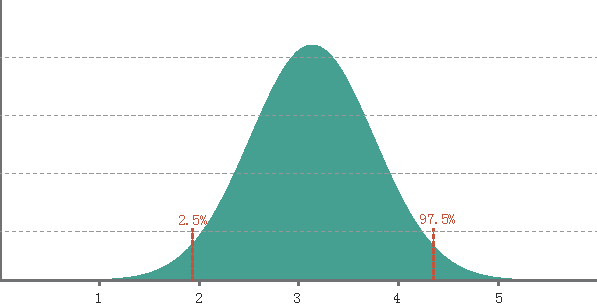
\includegraphics[width=.65\linewidth]{normalDistribution.pdf}}
\put(4.93,.5){
\includegraphics[width=1.29cm]{location.pdf}}
\put(10.7,.5){
\includegraphics[width=1.29cm]{diversity30.pdf}}
\put(10.7,4.5){\parbox{2cm}{\color{topcolor}\bfseries 您的数值高\\于33.70{\%}\\的参考人群。}}
\put(0,-.5){肠道菌群多样性分布图(紫色虚线标示了您的位置,红色虚线之间是参考区域)}
\end{picture}

\end{center}

\vspace{-1.2cm}
\begin{LRaside}[.8]{结果分析}
\noindent
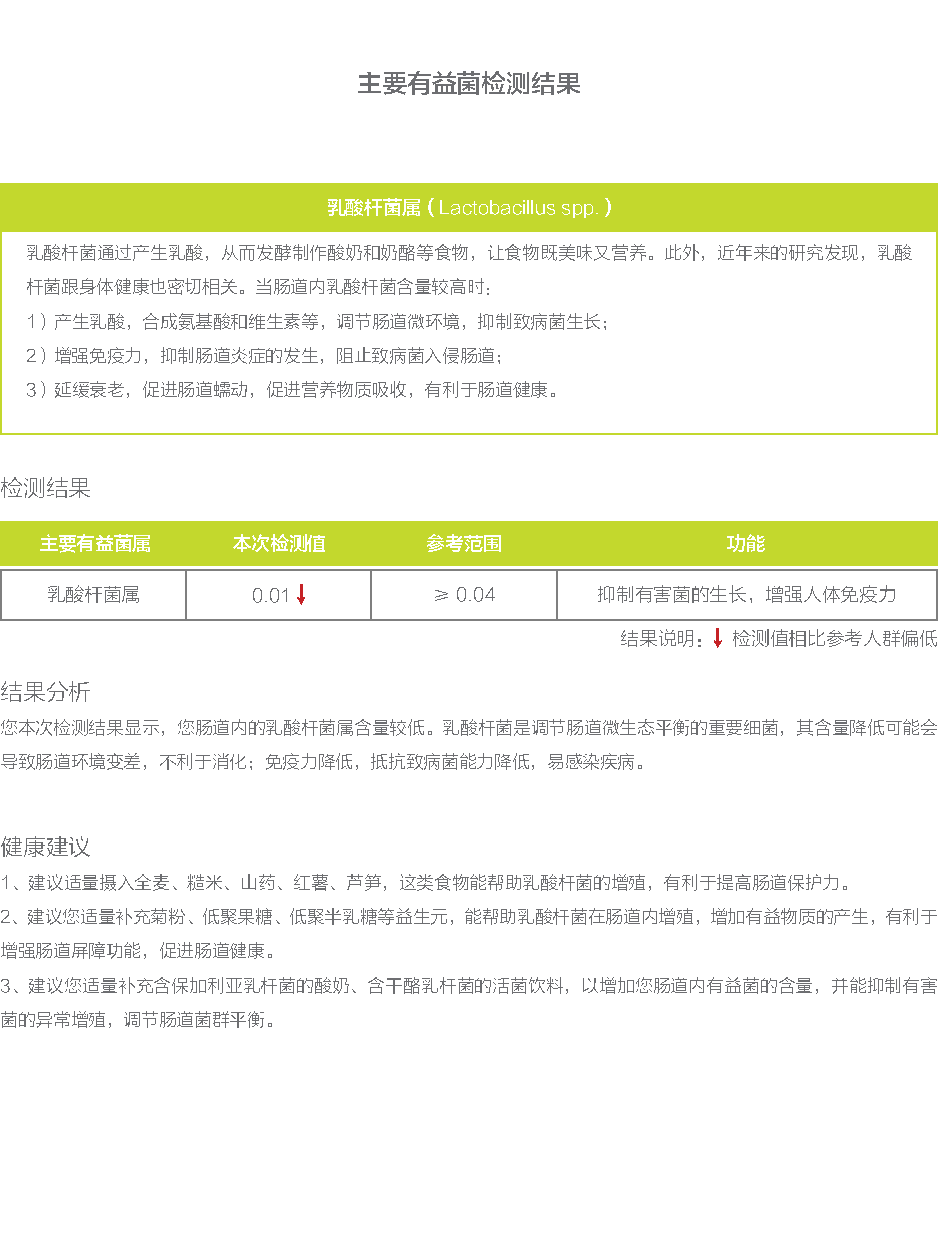
\includegraphics[width=\linewidth]{result.pdf}
\asidebreak %
您的肠道菌群多样性偏低,说明您的肠道菌群组成较为单一,菌群失调风险较高。您的肠道菌群较易受到外界因素的干扰(如不良作息、刺激性食物、药物滥用),可能会导致菌群失调,引起胃肠道炎症、免疫力低下、胰岛素抵抗等多种健康问题。
\end{LRaside}

\end{document}

